% Document uses 12 pt font
% 1 in margins
% Contains a relative path for images

\documentclass [10pt]{article}

% page geometry 
\usepackage[margin=1in]{geometry}


% ----------  PACKAGES START ------------ %
% Math Packages
\usepackage{amsmath}
\usepackage{mathtools}

% Table cell color package and highlighting
\usepackage[table]{xcolor}
\usepackage{color,soul}

% VIC title package
%\usepackage{cabin}
\usepackage[T1]{fontenc}

% default font package
%\usepackage{times}
\usepackage{helvet}
%\renewcommand{\familydefault}{\sfdefault}

% ---------- End Font Packages -------------- %

\usepackage{listings}


\definecolor{dkgreen}{rgb}{0,0.6,0}
\definecolor{gray}{rgb}{0.5,0.5,0.5}
\definecolor{mauve}{rgb}{0.58,0,0.82}

\lstset{frame=tb,
  language=C++,
  aboveskip=3mm,
  belowskip=3mm,
  showstringspaces=false,
  columns=flexible,
  basicstyle={\small\ttfamily},
  numbers=none,
  numberstyle=\tiny\color{gray},
  keywordstyle=\color{blue},
  commentstyle=\color{dkgreen},
  stringstyle=\color{mauve},
  breaklines=true,
  breakatwhitespace=true,
  tabsize=3
}

% Title Packages
\usepackage{titlesec}
\usepackage{titletoc}

% Image Package
\usepackage{graphicx}

% Table Packages
\usepackage{longtable}
\usepackage{multirow}
\usepackage{multicol}
\usepackage{multirow}
\usepackage{array}
\renewcommand{\arraystretch}{1.2}% Spread rows out evenly in table
\setlength{\LTpre}{0.5pt} % Reduces white space around tables (top)
%\setlength{\LTpost}{0pt} % Reduces white space around tables (bottom)

% Color Packages
\usepackage{color}   
\definecolor{sectionC}{rgb}{0.95,0.52,.0}
\definecolor{subsectionC}{rgb}{1.0,.64,.26}
\definecolor{subsubsectionC}{rgb}{1.0,.87,.68}
\definecolor{tableCell}{rgb}{.98,.81,.69}


% List package
\usepackage{enumitem}
\setenumerate{itemsep=0pt, itemindent=0in,leftmargin=0.5in}


% Paragraph parameter

\setlength{\parindent}{0pt}


% ------------- Creates a linked Table of Contents  Start --------------- %
\usepackage{hyperref}
\hypersetup{
colorlinks=true, %set true if you want colored links
linktoc=all,     %set to all if you want both sections and subsections linked
linkcolor=black,}  %choose some color if you want links to stand out

% ------------- Creates a click-able Table of Contents  End--------------- %

% ---------- PACKAGES END ------------ %








% -------- SECTION AND SUBSECTION FORMATING START -------- % 
% starts the 
%\setcounter{section}{1}


\titleformat{\section} % Section
{\normalfont \fontsize{14}{14} \bfseries}{}{0em}{\colorsection}

% Makes a background color
\newcommand{\colorsection}[1]{%
  \colorbox{sectionC}{\parbox{\dimexpr\textwidth-1\fboxsep}{\color{white}\Large\thesection\ \hspace{1mm} #1}}}

% Makes a background color
\titleformat{\subsection} % Subsection
{\normalfont \fontsize{12}{12}  \bfseries}{}{0em}{\colorsubsection }

\newcommand{\colorsubsection}[1]{%
  \colorbox{subsectionC}{\parbox{\dimexpr \textwidth -1\fboxsep}{\large\thesubsection\ #1}}}


% Makes a background color
\titleformat{\subsubsection} % Subsubsection
{\normalfont \fontsize{12}{12} \bfseries}{}{0em}{\colorsubsubsection}

\newcommand{\colorsubsubsection}[1]{%
  \colorbox{subsubsectionC}{\parbox{\dimexpr\textwidth-1\fboxsep}{\thesubsubsection\ #1}}}

% -------- SECTION AND SUBSECTION FORMATING END -------- % 
\usepackage{lipsum}


% -----  IMAGE PATH START -----%
% Relative Image Path
\graphicspath {figures/}
% -----  IMAGE PATH END -----%

% ------ PARAGRAPH FORMAT START ----%
%\setlength{\parskip}{.2em}% Sets the space between new paragraph items 
\setlength{\parindent}{0em} % paragraph indent
% ------ PARAGRAPH FORMAT END ----%




%------------------------------TOC FORMAT START --------------------------------%
\usepackage{tocloft}



% Section indentations
\cftsetindents{section}{0em}{1.5em}
\cftsetindents{subsection}{1em}{2em}
\cftsetindents{subsubsection}{2em}{3em}

% Toc title size
\renewcommand\cfttoctitlefont{\Large\bfseries}
\renewcommand*\contentsname{Table of Contents}

\newcommand{\carSpeed}{1.4\ m/s}
\newcommand{\intersectionLength}{0.6\ m}


% Removes bold headings from toc
%\renewcommand{\cftsecfont}{\normalfont}

% Removes bold heading page numbers from toc
\renewcommand{\cftsecpagefont}{\normalfont}

% add dots after headings
%\renewcommand{\cftsecleader}{\cftdotfill{\cftdotsep}} 


% number of section headings we want to see in toc
\setcounter{tocdepth}{2}

% Spaceing before headings in toc
\setlength{\cftbeforesecskip}{6pt}

% ------------------------------TOC FORMAT END --------------------------------%



% ------------------- START HEADER AND FOOTER ---------------------------%
\usepackage{fancyhdr}

% Helps with the n of total n pages
\usepackage{lastpage}

\pagestyle{fancy}

% Header
\lhead{Draft Component Design }
\rhead{Revision: 0}
\fancyhead[LE,CO]{Group 9: LazyBots}

% Removes line under the header 
\renewcommand{\headrulewidth}{0pt}
\setlength{\headsep}{.2in}

% Footer 

% Set the right side of the footer to be the page number
\fancyfoot[R]{Page \textbf{\thepage}\ of \textbf{\pageref{LastPage}}}
\fancyfoot[C]{}

% ------------------- END HEADER AND FOOTER ---------------------------%






% -------------- DOCUMENT START ---------------%
\begin{document}

% --------- TITLE PAGE START ------- %
\begin {center} 

\thispagestyle{empty}
\vspace*{5cm}

% Logo Insertion
\begin {figure}[h!]
\centering
\hspace{-10mm}
\includegraphics [scale = .3, trim={.4cm 0 .8cm 0},clip] {figures/alfred.png}
\end {figure}

{%\fontfamily{\cabinfamily}\selectfont
\Huge{LazyBots} }

\vspace{1 cm}
{\Large\textbf{\textsc{McMaster University}}\\}  \vspace {1cm}
{\Large Development Process and Implementation\\ \vspace {0.4 cm} SE 4GA6 \& TRON 4TB6}  \vspace {1cm}

{\large \textsc{Group 9} \\} \vspace{1cm}



\begin{tabular}{ l c  l}
Karim Guirguis & & 001307668 \\
David Hemms & & 001309228 \\
Marko Laban & & 001300989 \\
Curtis Milo & & 001305877 \\
Keyur Patel & & 001311559 \\
Alexandra Rahman & & 001305735
\end{tabular}


\end{center}


% --------- TITLE PAGE END------- %

\pagebreak

% Inserting table of contents and table of figures 

\tableofcontents
\listoftables
\listoffigures



\pagebreak

% -----------  REVISION HISTORY START ----------- %

%\section*{Revisions}
\thispagestyle{empty}
\section{Revisions}
\begin{longtable}{| p{.2\textwidth } | p{.23\textwidth } | p{.23\textwidth } | p{.23\textwidth } |} \caption{VIC Table of Revisions}  \\

% ------------------------------------------------------- Date ------------------------------------------------------- %
\hline 
\centering \textbf{Date} & 
\multicolumn{1}{c}{\textbf {Revision Number}} &
\multicolumn{1}{|c}{\textbf {Authors}} & 
\multicolumn{1}{|c|}{\textbf {Comments}} \\ \hline

% ------------------------------------------------------- Revision Number -------------------------------------------------------
\multirow{4}{*}{\centering November 24\textsuperscript{th}, 2017}  & 
\multirow{4}{*}{Revision 0}& 
		{Karim Guirguis \newline
		David Hemms \newline
		Marko Laban \newline
		Curtis Milo \newline
		Keyur Patel \newline
		Alexandra Rahman}
 &
 
% ------------------------------------------------------- Comments -------------------------------------------------------
\multirow{4}{*}{-} \\ 
\hline 

\end{longtable}



\pagebreak

%---------------------------- PROJECT DRIVERS ------------------------%
% heading in document

% -------------- START INTRODUCTION ---------------- %


\section {Purpose}

The purpose of this project will be to create an autonomous robot that will navigate to and serve
the requested drink to the user who requests a drink. Currently in an office setting, workers must
leave their offices to get their own drinks. Also, in restaurants, drinks are served by waiters and
waitresses, which hinders them from doing other work at that time. Alfred will be designed to make the serving drinks autonomous.\newline

Alfred will allow users to request drinks. These requests will form a queue which Alfred will serve in order using a FIFO protocol. Alfred will go to the table of each user and pour the drinks ordered from that table. Alfred will also have an administrator user which will be able to call Alfred back and override any action that is being taken at the time.\newline

The following document will outline the overall system components, as well as the overall system behaviour, operation and undesired error handling.

\subsection{Scope}

The system implemented is one that is meant to automate the dispensing of beverages to customers within a restaurant at the respected customers' table. The customer will be able to order a drink from their table which will be followed by Alfred arriving at their table and dispensing the requested drinks. The staff will be able to request Alfred to come back for charging and refilling when desired.


\subsection{Context Diagram}
The following is a context diagram of the drink serving robot, Alfred.
\begin{figure} [h!]
	\centering
	\includegraphics [scale = 0.6] {Figures/ContextDiagram.png}
	\caption{Drink Serving Robot Context Diagram}
\end{figure}

\subsection{Diagram of Components}
The following is a diagram that shows the interaction of components of the drink serving robot system.
\begin{figure} [h!]
	\centering
	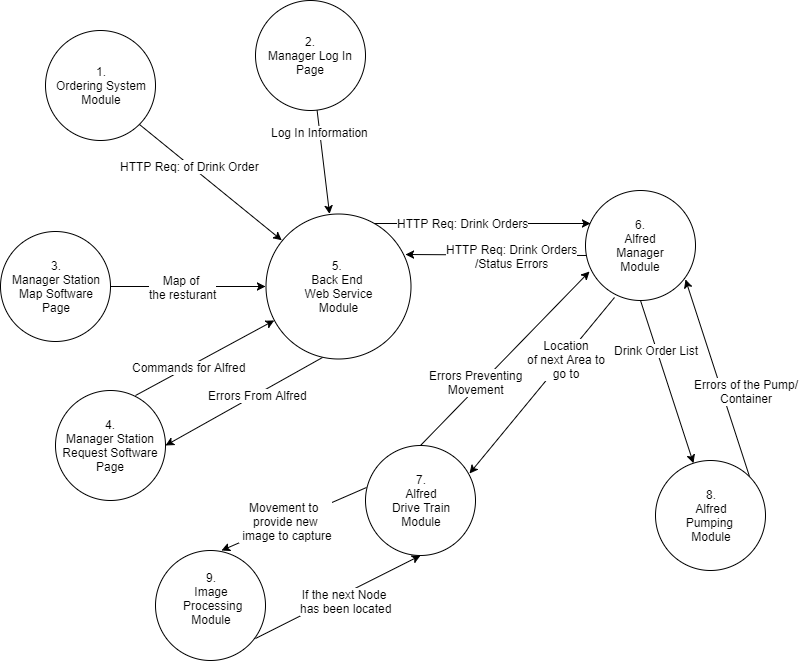
\includegraphics [scale = 0.6] {Figures/SystemComponents.png}
	\caption{Drink Serving Robot System Component Diagram}
\end{figure}
\section{System Variables}

\subsection{Monitored and Controlled Variables}
The following is a list of variables that will be monitored.

\begin{longtable}{|l|l|l|l|l|}\hline 
	\rowcolor{tableCell}Monitor Name & Monitor Type & Range & Units & Comment(s) \\ \hline
	$ w_{wheel_{left}} $ & Speed & [0, $ 100 $]& rad/s &  Left Wheel Speed\\ \hline
	$ w_{wheel_{right}} $ & Speed & [0, $ 100 $]& rad/s & Right Wheel Speed \\ \hline
	$ m_{container} $ & Mass & [0, 1.0]& Kg &  Weight of the storage device  \\ \hline
	$ m_{drink} $    & Mass & [0, 1.0] & Kg &  Weight of the drink  \\ \hline
	$ b_{cuptaken } $ & Boolean & [0,1] & N/A & If the cup has been taken \\ \hline
	$  d_{objects} $ & Distance[] & [0, 10.0]& m & Set of distances to closest obstacle \\ \hline
	$  V_{batt} $ & Voltage & [0, 20.0]& m &  Voltage levels of batteries \\ \hline
\end{longtable}


The following is a list of variables that will be controlled

\begin{longtable}{|l|l|l|l|l|}\hline 
	\rowcolor{tableCell}Controlled Name & Controlled Type & Range & Units & Comment(s) \\ \hline
    $w_{motor}$ & Speed & [0, $ 100 $]& rad/s &  Motor Speed\\ \hline
    	$ percent_{dutycycle_{left}} $ & Percent & [0,1.0] & \% & The duty cycle of the left side of the drive-train \\ \hline
    $ percent_{dutycycle_{right}} $ & Percent & [0, 1.0]& \% & The duty cycle of the right side of the drive-train\\ \hline
    $  V_{pump} $ & Voltage & [0, 5.0]& m &  Voltage going to the liquid pump \\ \hline
	$ errors_{drivetrain} $ & Unsigned Byte & [0, $2^{8}$]& N/A & Errors from drive-train \\ \hline
	$  errors_{pump} $ & Unsigned Byte & [0, $2^{8}$]& N/A & Errors from pumping system module \\ \hline
	$  errors_{Alfred} $ & Unsigned Byte & [0, $2^{8}$]& N/A & Errors from Alfred \\ \hline
	$LED_{drinksignal}$ & Boolean & [0, 1]& N/A & Signal of drink that it is ready to be picked up \\ \hline
	$Q_{pump}$ & Flow Rate & [0, $ 100 $]& ($m^3/s$) &  Flow rate of the pump\\ \hline
\end{longtable}



\begin{longtable}{|l|l|l|l|l|}\hline 


\end{longtable}

\subsection{Constants}

The following is a list of system constants

\begin{longtable}{|l|l|l|l|l|}\hline 
	\rowcolor{tableCell}Constant Name & Constant Type & Value & Units & Comment(s) \\ \hline
 	$ V_{battMin} $ & Voltage & 9.0& m &  The minimum voltage necessary for drive-train movement \\ \hline
	$ m_{DrinkMin} $ & Mass & 0.35 & Kg &  The minimum weight of the drink to be considered as ready for the customer.  \\ \hline
	$ t_{timeout} $ & Time & 30 & s & The maximum time Alfred or the ordering application will wait for a message from the server before timing out.  \\ \hline
	$ t_{pumptimeout} $ & Time & 5 & s & The maximum time Alfred will try to pump without noticing a change in the weight of the tank.  \\ \hline
	$ t_{maxpump} $ & Time & 10 & s & The maximum time Alfred will try to dispense a drink within. \\ \hline
	$Q_{pump}$ & Flow Rate & TBD & ($m^3/s$) &  Flow rate of the pump\\ \hline
	$ freq_{bauderate} $ & Frequency & 9600 & (Herts) &  The  rate at which UART communication will be performed at.\\ \hline
	$ obstruction_{timeout} $ & Time & 10 & s & The amount of time that Alfred will stop movement due to an object in its path before ruling that there is an obstruction and throwing an error. \\ \hline
\end{longtable}



\section{Behaviour Overview}
\begin{enumerate}
	\item \textbf{Ordering System Module} - Provided the order information, this module will communicate with the server to "order a drink".
	\item \textbf{Manager Login Page} - Given the login credentials, will authenticate administrator of the system with the server.
	\item \textbf{Manager Station Map Software Page} - Will allow administrator to create/modify the map of the area where Alfred will deliver drinks. This map will then be sent and stored on the server.
	\item \textbf{Manager Station Request Software Page} - Will allow administrator to execute commands for Alfred, as well as view incoming error codes from Alfred. Said commands, will be sent to the server, which will then communicate with Alfred.
	\item \textbf{Back End Web Service Module} - Will route communication to different components of the system. Also will be responsible for authentication and management of queue. 
	\item \textbf{Alfred Manager Module} - Endpoint for communication with Alfred. Will manage communication with server, as well as send any errors that Alfred is experiencing.
	\item \textbf{Alfred Drive Train Module} - Responsible for driving and managing the motors based on desired route. Also, will be send errors preventing movement to Alfred Manager Module.
	\item \textbf{Alfred Pumping Module} - Will control pumping system in regards of when to pour, how long, rate of dispensing, etc. Also, will be send errors of pump/container to Alfred Manager Module.
	\item \textbf{Image Processing Module} - Will detect any obstacles in the way as well as locate incoming nodes. Will communicate with Alfred Drive Train Module, to determine any required action based on results.
\end{enumerate}

\section{Component Overview}
\subsection{Ordering System Module}

\subsubsection{Inputs and Outputs}

\textbf{Inputs: }  User input defining:

\begin{longtable}{|l|l|l|l|l|}\hline 
	\rowcolor{tableCell}Input Name & Input Type & Range & Units & Comment(s) \\ \hline
	$Order_{Num} $ & Unsigned Integer User Input & [0,5] & count &  Number of Orders \\ \hline
	$Order_{Drinks} $ &  User Input & N/A & N/A &  List of Ordered Drinks \\ \hline
\end{longtable}


\textbf{Outputs: } Packaged Information within HTTP Request for:
\begin{longtable}{|l|l|l|l|l|}\hline 
	\rowcolor{tableCell}Output Name & Output Type & Range & Units & Comment(s) \\ \hline
	$Order_{Num} $ & Unsigned Integer User Input & [0,5] & count &  Number of Orders \\ \hline
	$Order_{Drinks} $ &  User Input & N/A & N/A &  List of Ordered Drinks \\ \hline
	$Order_{TableNum} $ & Unsigned Integer User Input & [0,$2^{16}$] & N/A &  Table Number \\ \hline
	$Order_{Rid} $ & Unsigned Integer User Input & [0,$2^{16}$] & N/A & Identification of the restaurant \\ \hline
\end{longtable}
\subsubsection{Description}
This module will be used as the user input to take orders of the client. This user input will be taken in by the mobile application based on different button inputs/ radio button selections. These orders are then packaged by the module to be sent to the server based on an HTTP request.

\subsubsection{Timing Constraints}
Timing Constraints are based on the server sending a success signal within $ t_{timeout} $ seconds.

\subsubsection{Initialization}
At startup/new order of the application, it will start a blank order page where the user will be able to add drink orders and use radio buttons to select the desired drink.

\subsection{Manager Login Page Module}

\subsubsection{Inputs and Outputs}



\textbf{Inputs: } 

\begin{longtable}{|l|l|l|l|l|}\hline 
	\rowcolor{tableCell}Input Name & Input Type & Range & Units & Comment(s) \\ \hline
	$  UserName $ & String User Input & 10 chars & N/A & \\ \hline
	$  Password $ & String User Input & 20 chars  & N/A & \\ \hline
	$  GotoMapPage $ & Button User Input & [0,1]  & N/A & \\ \hline
	$  GotoAlfredInfo $ & Button User Input & [0,1]  & N/A & \\ \hline
\end{longtable}


\textbf{Outputs: } To be displayed to the user
\begin{longtable}{|l|l|l|l|l|}\hline 
	\rowcolor{tableCell}Output Name & Output Type & Range & Units & Comment(s) \\ \hline
	$  FailureMessage $ & String & 10 chars & N/A & Failure message if there is an incorrect information  \\ \hline
	$  GotoPage $ & Action & N/A  & N/A & navigating to the correct page if it was a success. \\ \hline
\end{longtable}

\subsubsection{Description}
This module is a web based application for the managers to be able to log into the management systems.
\subsubsection{Timing Constraints}
Given optimal networking conditions, the server must respond with $ t_{timeout} $ seconds.

\subsubsection{Initialization}
This will default to a HTML page with no information.


\subsection{Manager Station Map Software Module}

\subsubsection{Inputs and Outputs}

\textbf{Inputs: } User input defining:

\begin{longtable}{|l|l|l|l|l|}\hline 
	\rowcolor{tableCell}Input Name & Input Type & Range & Units & Comment(s) \\ \hline
	$ Resturant_{Width} $ & Integer User input &  [0,20] & m &  \\ \hline
	$ Resturant_{Length} $ & Integer User input &  [0,20] & m &  \\ \hline
	$ Resturant_{CanTravel[][]} $ & Button[][] User input &  N/A & N/A & A set of areas in which Alfred can travel to \\ \hline
	$ Resturant_{Tables[][]} $ & Button[][] User input &  N/A & N/A & A set of areas in which contains tables \\ \hline
	$ Resturant_{CannotTravel[][]} $ & Button[][] User input &  N/A & N/A & A set of areas in which Alfred cannot travel to \\ \hline
	$ Resturant_{Home} $ & Button User input &  N/A & N/A & An area that defines Alfred's home location \\ \hline
\end{longtable}


\textbf{Outputs: }A text file that contains the following information
\begin{longtable}{|l|l|l|l|l|}\hline 
	\rowcolor{tableCell}Input Name & Input Type & Range & Units & Comment(s) \\ \hline
	$ Resturant_{Width} $ & Integer &  [0,20] & m &  \\ \hline
	$ Resturant_{Length} $ & Integer  &  [0,20] & m &  \\ \hline
	$ Resturant_Data $& Char  &  [H,X,0,T] & N/a & Table Information \\ \hline
\end{longtable}


\subsubsection{Description}
This module will be used as the user input to create a map where the manager of the restaurant will be able to define the details about the restaurant that will help Alfred with it's navigation to different tables.

\subsubsection{Timing Constraints}
Timing Constraints are based on the server sending a success signal within  $ t_{timeout} $ seconds.

\subsubsection{Initialization}
At startup/new order of the application, it will load in the users map that is associated with their profile. If this is the first time using the application then it will default to a 1x1 map.

\subsection{Manager Station Request Software Module}

\subsubsection{Inputs and Outputs}

\textbf{Inputs: } 

\begin{longtable}{|l|l|l|l|l|}\hline 
	\rowcolor{tableCell}Input Name & Input Type & Range & Units & Comment(s) \\ \hline
	$ req_{Home} $ & Boolean User input &  [0,1] & N/A & Calling back Alfred \\ \hline
	$  errors_{Alfred} $ & Unsigned Byte & [0, $2^{8}$]& N/A & Errors from Alfred \\ \hline
\end{longtable}


\textbf{Outputs: } To be displayed to the User
\begin{longtable}{|l|l|l|l|l|}\hline 
	\rowcolor{tableCell}Output Name & Output Type & Range & Units & Comment(s) \\ \hline
	$  warn_{LowLiquid} $ & Boolean & [0, 1]& N/A & Low liquid levels \\ \hline
	$  error_{LiquidLeak} $ & Boolean & [0, 1]& N/A & Leaking of liquid error \\ \hline
	$  error_{NotPumping} $ & Boolean & [0, 1]& N/A & Not pumping error \\ \hline
	$  error_{NoMovement} $ & Boolean & [0, 1]& N/A & Not able to move error \\ \hline
	$  error_{LowBatt} $ & Boolean & [0, 1]& N/A & Low battery Error \\ \hline
\end{longtable}
\subsubsection{Description}
This module is used for the manager to determine the state of Alfred from an office as well as being able to override the robot to come back to the home base. 
\subsubsection{Timing Constraints}
One timing constraints are based on the server sending a success signal within  $ t_{timeout} $ seconds. Another constraint is that Alfred will return within the time of $ w_{wheel} $*distance.

\subsubsection{Initialization}
At startup this interface should pull the last status of the robot and display it to the user. If no previous data is found then it will return that there are currently no errors.

\subsection{Back End Web Service Module}

\subsubsection{Inputs and Outputs}

\textbf{Inputs: } 

\begin{longtable}{|l|l|l|l|l|}\hline 
	\rowcolor{tableCell}Input Name & Input Type & Range & Units & Comment(s) \\ \hline
	$ HttpReq_{Orders} $ & HTTP Request & N/A & N/A & HTTP request package with the information for drink orders. \\ \hline
	$ Map_{textfile} $ & Text File & N/A & N/A & A text file with a map \\ of the restaurant \\ \hline
	$  errors_{Alfred} $ & Unsigned Byte & [0, $2^{8}$]& N/A & Errors from Alfred \\ \hline
	$  UserName $ & String & 10 chars & N/A & \\ \hline
	$  Password $ & HashCode & N/A & N/A &  Success result for authenticated results. \\ \hline
\end{longtable}


\textbf{Outputs: } 
\begin{longtable}{|l|l|l|l|l|}\hline 
	\rowcolor{tableCell}Output Name & Output Type & Range & Units & Comment(s) \\ \hline
	$ HttpReq_{Orders} $ & HTTP Request & N/A & N/A & HTTP request package with the information for drink orders. \\ \hline
	$ Map_{textfile} $ & Text File & N/A & N/A & A text file with a map \\ of the restaurant \\ \hline
	$  errors_{Alfred} $ & Unsigned Byte & [0, $2^{8}$]& N/A & Errors from Alfred \\ \hline
	$  Login_{Status} $ & String & 10 chars & N/A & Login Success or Fail \\ \hline
	$  Http_{Result} $ & String & 10 chars & N/A & \\ \hline
\end{longtable}

\subsubsection{Description}
This module is a server component that will hold account information for different restaurants. This will perform authorize different users to be able to accept different drink requests from the ordering system. It will return the next drink order for the restaurants Alfred robot.
\subsubsection{Timing Constraints}
Given optimal networking conditions, the server must respond with  $ t_{timeout} $ seconds.

\subsubsection{Initialization}
This server will be initialized by a database with one restaurant which will be used for the purposes of testing the system

\subsection{Alfred Manager Module}

\subsubsection{Inputs and Outputs}


\textbf{Inputs: } 

\begin{longtable}{|l|l|l|l|l|}\hline 
	\rowcolor{tableCell}Input Name & Input Type & Range & Units & Comment(s) \\ \hline
	$ Map $ & Graph & N/A & N/A & Graph of the text file with a map \\ of the restaurant \\ \hline
	$ Orders_{drinks} $ & Order[] & N/A & N/A & A list of drink orders ordered by table. \\ \hline
	$ b_{requestHome} $ & Boolean & [0, 1]& N/A &  A request to come back to the base\\ \hline
	$ errors_{drivetrain} $ & Unsigned Byte & [0, $2^{8}$]& N/A & Errors from drive-train \\ \hline
	$  errors_{pump} $ & Unsigned Byte & [0, $2^{8}$]& N/A & Errors from pumping system module \\ \hline
\end{longtable}


\textbf{Outputs: } 
\begin{longtable}{|l|l|l|l|l|}\hline 
	\rowcolor{tableCell}Output Name & Output Type & Range & Units & Comment(s) \\ \hline
	$ NextOrder $ & Order & N/A & N/A & Next Drink Order. \\ \hline
	$ NextNode $ & Node & [(0,0), (length($Map)$,width($Map$)] & N/A & The next node to travel to. \\ \hline
	$  errors_{Alfred} $ & Unsigned Byte & [0, $2^{8}$]& N/A & Errors from Alfred \\ \hline
\end{longtable}

\subsubsection{Description}
This module acts as the manager to the different components of Alfred. It will run on a raspberry pi to command the drive-train to move to different nodes of the map. The manager will also communicate through UART to the different on board micro-controller for commanding the next drink to the pumping system.
\subsubsection{Timing Constraints}
Given optimal networking conditions, the system must receive a response within  $ t_{timeout} $ seconds. The communication with the pumping system must be done at the specified $freq_{bauderate}$.

\subsubsection{Initialization}
This will assume that there is no requests at startup. It will request from the server asking for the next drink order. If there is no map previously defined within a text file then it will request this as well.

\subsubsection{Alfred Communication Circuit Diagram}
The following is a circuit diagram showing the communication between the Raspberry Pi and the pumping system.
\begin{figure} [h!]
	\centering
	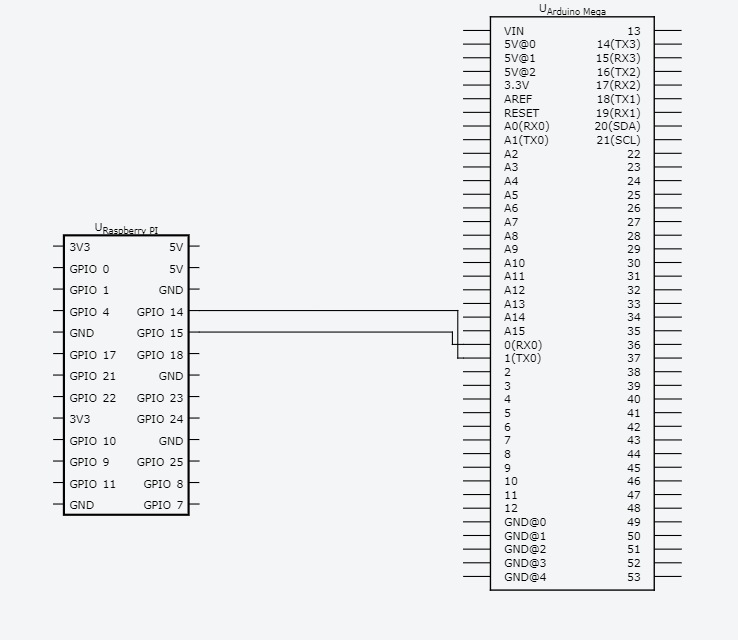
\includegraphics [scale = 0.6] {Figures/UART.png}
	\caption{Alfred Communication Circuit Diagram}
\end{figure}

\subsubsection{Raspberry PI Specifications}
Manufacturer: Raspberry PI \\
Processor: Broadcom BCM2387 chipset. \\
Memory: 1GB \\
Power:Micro USB socket 5V1, 2.5A\\
GPIO: 17 pins as well as +3.3 V, +5 V and GND supply lines\\
Camera Connector: 15-pin MIPI Camera Serial Interface (CSI-2)\\
Memory Card Slot: Push/pull Micro SDIO\\

\subsection{Alfred Drive-train Module}

\subsubsection{Inputs and Outputs}

\textbf{Inputs: } 


\begin{longtable}{|l|l|l|l|l|}\hline 
	\rowcolor{tableCell}Input Name & Input Type & Range & Units & Comment(s) \\ \hline
	$ Map $ & Graph & N/A & N/A & Graph of the text file with a map \\ of the restaurant \\ \hline
	$ NextNode $ & Node & [(0,0), (length($Map)$,width($Map$)] & N/A & The next node to travel to. \\ \hline
	$ w_{wheel_{left}} $ & Float & [0, $ 100 $]& rad/s &  Left Encoder Input\\ \hline
	$ w_{wheel_{right}} $ & Float & [0, $ 100 $]& rad/s & Right Encoder Input  \\ \hline
	$  d_{objects} $ & Float[] & [0, 10.0]& m &  \\ \hline
	$ Marker_{PosX} $ & Unsigned Integer & [0,$2^{16}$] & Pixels &  \\ \hline
	$ Marker_{PosY} $ & Unsigned Integer & [0,$2^{16}$] & Pixels & \\ \hline
	$ b_{NextMarkerFound} $ & Boolean & [0,1] & N/A & \\ \hline
	$  V_{batt} $ & Float & [0, 20.0]& m &  \\ \hline
\end{longtable}


\textbf{Outputs: } 
\begin{longtable}{|l|l|l|l|l|}\hline 
	\rowcolor{tableCell}Output Name & Output Type & Range & Units & Comment(s) \\ \hline
	$ percent_{dutycycle_{left}} $ & Float & [0,1.0] & \% &  \\ \hline
	$ percent_{dutycycle_{right}} $ & Float & [0, 1.0]& \% & \\ \hline
	$ errors_{drivetrain} $ & Unsigned Byte & [0, $2^{8}$]& N/A & \\ \hline
\end{longtable}

\subsubsection{Description}
This module will provide power to the drive-train of Alfred. It will use the feedback of the left and right encoders and take the error to perform PI control on them. This PI control output will then be translated into a duty cycle for each side to be able to power the DC motors with pulse width modulation. This module will communicate to the image recognition software to receive the position of the next next marker and use this information of where it currently is on its path. This module will use ultrasonic sensors to get a set of distances ($ d_{object} $) to the nearest object to determine if it is safe to continue moving.

\subsubsection{Timing Constraints}
This module will have to deliver speed requirements that of walking speed so that it will be able to serve tables at a timely manner.

\subsubsection{Initialization}
This module will not be started until manager starts the process and initializes the proper information.


\subsubsection{Diagram of Simulink Control System}
The following is a diagram that shows the top level of the dc motor control system. 
\begin{figure} [h!]
	\centering
	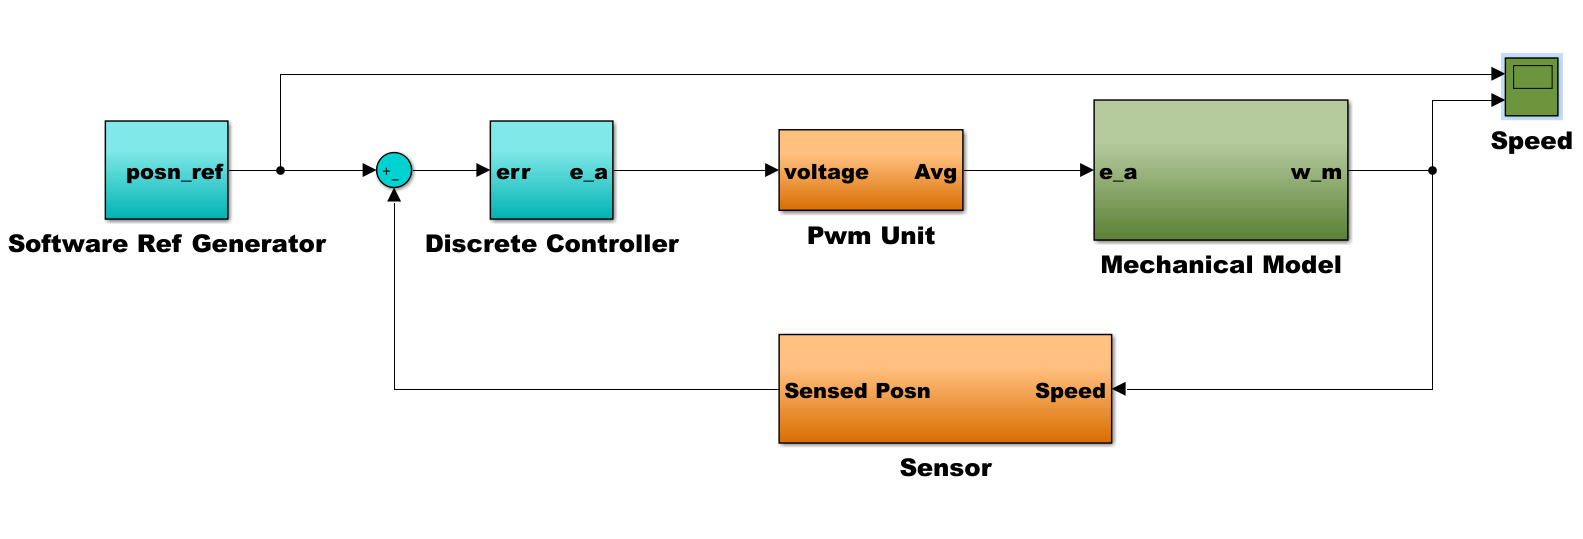
\includegraphics [scale = 0.6] {Figures/Simulink.png}
	\caption{Top level of the dc motor control system}
\end{figure}

\subsubsection{DC Motors Circuit Diagram}
The following is a circuit diagram for showing the DC motor drive-train.
\begin{figure} [h!]
	\centering
	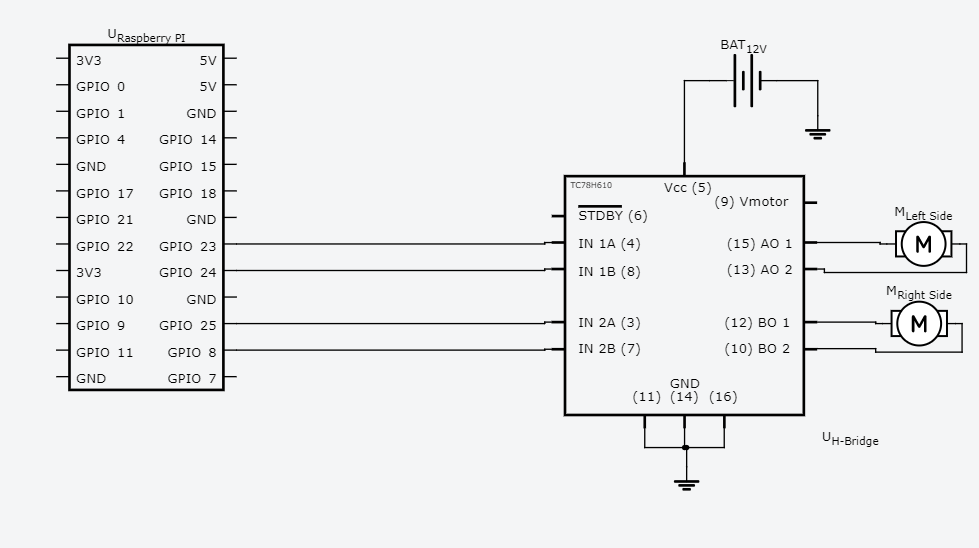
\includegraphics [scale = 0.6] {Figures/H_Bridge.png}
	\caption{Weight Detection Circuit Diagram}
\end{figure}

\subsubsection{DC Motor Specifications}
Manufactured Part Number: 393111-01\\
Rated Voltage: 18V\\
Current: 3A-5A\\

\subsubsection{H-bridge Specifications}
Manufactured Part Number:  IRF3205\\
Rated Voltage: 3~36V \\
Rated Current: 10A continuous, Peak 30A \\

\subsubsection{Encoder Specifications}
Shaft Diameter 6mm\\
Working Range: 3-5V DC\\

\subsection{Alfred Pumping System Module}

\subsubsection{Inputs and Outputs}

\textbf{Inputs: } 

\begin{longtable}{|l|l|l|l|l|}\hline 
		\rowcolor{tableCell}Input Name & Input Type & Range & Units & Comment(s) \\ \hline
		$ b_{cuptaken } $ & Boolean & [0,1] & N/A &  \\ \hline
		$ m_{container} $ & float & [0, 1.0]& Kg & \\ \hline
		$ m_{drink} $    & float & [0, 1.0] & Kg &  \\ \hline
		$ Order_{drinks} $ & Order[] & N/A  & N/A & List of Drinks  \\ \hline
\end{longtable}
\textbf{Outputs: } 
\begin{longtable}{|l|l|l|l|l|}\hline 
	\rowcolor{tableCell}Output Name & Output Type & Range & Units & Comment(s) \\ \hline
	$ LED_{drinksignal} $ & Boolean & [0,1] & N/A &  \\ \hline
	$ V_{pump } $ & float & [0, 5.0]& V & \\ \hline
	$  errors_{pump} $ & Unsigned Byte & [0, $2^{8}$]& N/A & \\ \hline
\end{longtable}
\subsubsection{Description}
This module consists of an Arduino Mega which will receive information from the Alfred manager module through UART to receive the next drink order. This will then begin to dispense the specific drink until it has reached $ m_{containerMin} $. It will then show the customer that the drink has been completed by turning on: $ LED_{drinksignal} $. It will then read $ b_{cuptaken} $ from a light sensor to determine if the cup has been taken at which point it will then wait for the next drink cup to get in place and begin pouring. If it is not able to pump liquid, or it is losing fluid when not dispensing, then it will send the appropriate errors through UART back to the manager.

\subsubsection{Timing Constraints}
This module will have to dispense the drink within $ t_{maxpump} $

\subsubsection{Initialization}
This module start by waiting for the manager to send the drink information for the system to pour. All errors within the system will start as false until they have been triggered.

\subsubsection{Diagram of DC Pump Control System}
The following is a diagram that shows the top level of the dc pump control system. 
\begin{figure} [h!]
	\centering
	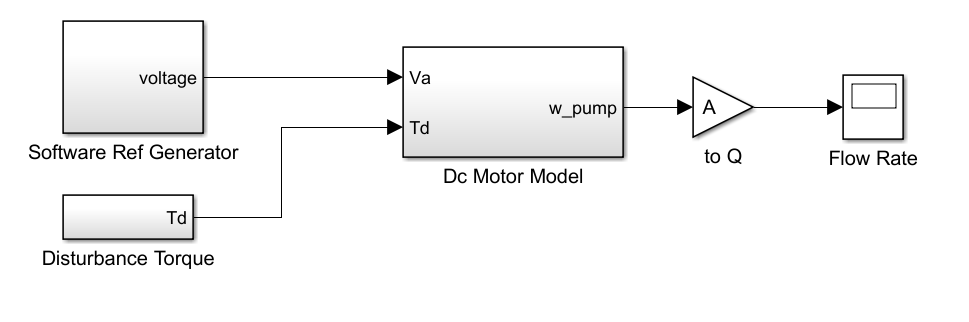
\includegraphics [scale = 0.6] {Figures/DC_PumpSim.png}
	\caption{Top level of the dc motor control system}
\end{figure}

\subsubsection{DC Pump Circuit Diagram}
The following is a diagram that shows the DC Pump Circuit.
\begin{figure} [h!]
	\centering
	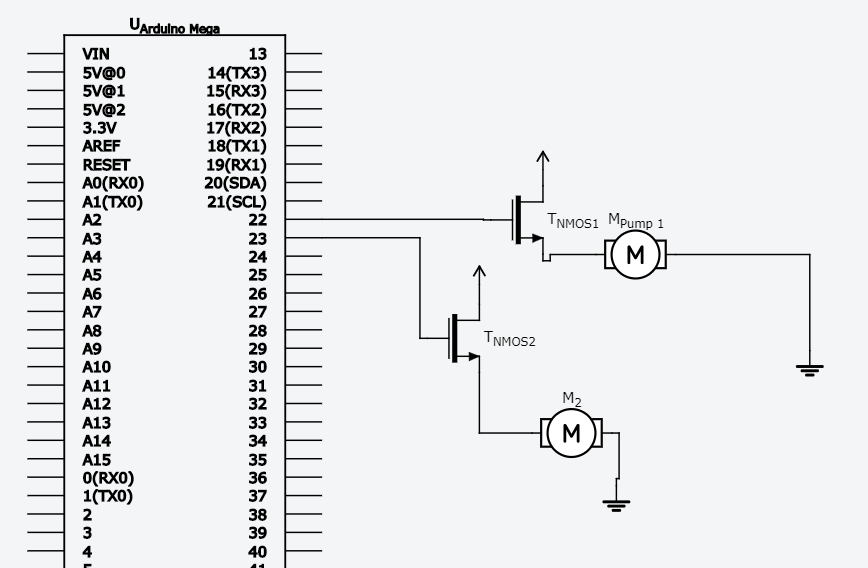
\includegraphics [scale = 0.6] {Figures/Pump.png}
	\caption{DC Pump Circuit Diagram}
\end{figure}


\subsubsection{Liquid Temperature Circuit Diagram}
The following is a circuit diagram for sensing the temperature of the liquid.
\begin{figure} [h!]
	\centering
	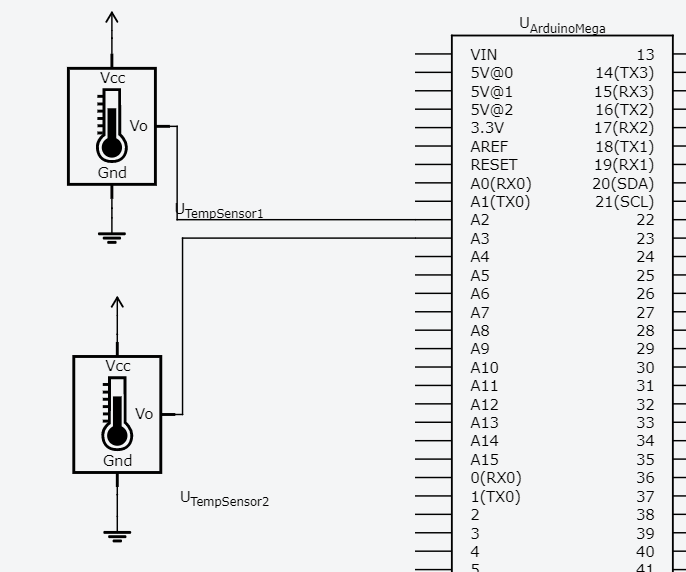
\includegraphics [scale = 0.6] {Figures/TempSensor.png}
	\caption{Top level of the dc motor control system}
\end{figure}


\subsubsection{Weight Detection Circuit Diagram}
The following is a circuit diagram for sensing the weight of the storage containers.
\begin{figure} [h!]
	\centering
	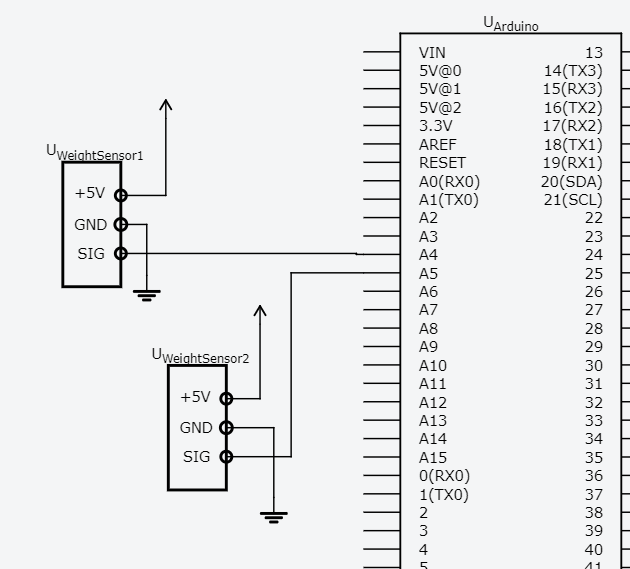
\includegraphics [scale = 0.6] {Figures/WeightSensors.png}
	\caption{Weight Detection Circuit Diagram}
\end{figure}


\subsubsection{DC Pump Specifications}
Manufacture : Yosoo \\
DC Voltage: 3-6V\\
Flow rate: 80-120L/H\\
Material: engineering plastic\\
Diameter: 24.5mm by 46mm \\
Outside diameter:  0.3" 

\subsubsection{Arduino Mega Specifications} 
Microcontroller:	ATmega1280\\
Operating Voltage:	5V\\
Digital I/O Pins: 54 (of which 15 provide PWM output)\\
Analog Input Pins: 16\\
DC Current per I/O Pin: 40 mA\\
DC Current for 3.3V Pin: 50 mA\\
Flash Memory: 128 KB\\
Clock Speed: 16MHz\\

\subsubsection{Container Specifications} 

Manufacture : Rubbermaid \\
Dimensions: 10 1/2" x 9" x 4" 
Capacity: 18 Cups/4.2 L\\
\subsubsection{Tubing Specifications}
Manufacture : Plumb Craft \\
Diameter: 1/4"ID Food Grade Tubing will be used.\\

\subsection{Alfred Image Processing Module Module}

\subsubsection{Inputs and Outputs}

\textbf{Inputs: } 

\begin{longtable}{|l|l|l|l|l|}\hline 
	\rowcolor{tableCell}Input Name & Input Type & Range & Units & Comment(s) \\ \hline
	 & Bitmap &  N/A & N/A & Image of the ceiling  \\ \hline
\end{longtable}

\textbf{Outputs: } 

\begin{longtable}{|l|l|l|l|l|}\hline 
	\rowcolor{tableCell}Output Name & Output Type & Range & Units & Comment(s) \\ \hline
	$ Marker_{PosX} $ & Unsigned Integer & [0,$2^{16}$] & Pixels &  \\ \hline
	$ Marker_{PosY} $ & Unsigned Integer & [0,$2^{16}$] & Pixels & \\ \hline
	$ b_{NextMarkerFound} $ & Boolean & [0,1] & N/A & \\ \hline
\end{longtable}

\subsubsection{Description}
This module will receive information from a camera while the drive-train is in motion. This camera will be looking at the ceiling looking for positions of circles that will denote one meter distances set up within a grid around the ceiling of the restaurant. This module will determine if there is a new maker within the image and if so where is the X and Y position of that marker to provide to the drive-train.

\subsubsection{Timing Constraints}
This information must process in time for the drive train to be able to navigate based off of it.

\subsubsection{Initialization}
This module start by the drive-train application.

\subsubsection{Raspberry PI Camera Specifications}
Manufacturer: Raspberry PI \\
Resolution: 1080p30, 720p60 and 640 × 480p60/90\\
Field of View (FOV): 62.2 degrees by 48.8 degrees\\

\section{Normal Operation}
Alfred is a mostly autonomous robot, only requiring human intervention in the event of an error or warning. Alfred will be able to navigate the restaurant by itself, and will serve drinks to tables. Customers will be able to place orders via a mobile application, which will be sent to a server. Orders to serve will be sent to Alfred using a FIFO protocol. Once Alfred has finished with an order, it will be able to request for a new order to serve. Management will be able to recall Alfred to the kitchen at any point using the admin console. In the event of a recall, Alfred will finish the current job and will return to the kitchen afterwards. Management will also be able to create a map of the restaurant and upload it to Alfred, which will give Alfred the means to navigate the restaurant.



\section{Undesired Event Handling}
Alfred will be able to detect undesired behaviours and conditions such as low liquid levels below threshold $ m_{containerMin} $, any issues with pumping liquid, low battery level, leaking liquids, and any blockages in the current path once Alfred has been blocked for a time greater than $ obstruction_{timeout} $. In the event of any error condition, Alfred will send an error code to the kitchen, to alert the staff of the issue. Wherever possible, Alfred will return to the kitchen in an error condition to request a fix. Otherwise, if movement is not possible, the kitchen staff will have to pick Alfred up from the dining room. Along with alerting management of any current errors, Alfred will also be able to indicate whether it is returning to the kitchen or requires pickup.

\section{References}


\textbf{Raspberry pi data sheet}
\begin{verbatim}
[1]"Exploring Raspberry Pi", 2017. [Online]. Available: http://docs-europe.electrocomponents.com/webdocs/14ba/0900766b814ba5fd.pdf. [Accessed: 23- Dec- 2017].
\end{verbatim}
\textbf{Arduino Mega Information}
\begin{verbatim}
[2] "Arduino Mega". [Online]. Available:
https://www.arduino.cc/en/Main/ArduinoBoardMega. [Accessed: 23- Dec- 2017].
\end{verbatim}
\textbf{DC Pump Information}
\begin{verbatim}
[3] "3-6V Mini Micro Submersible Pumps DC Motor Pump Water Pump - 80-120L/H". [Online]. Available:
https://www.amazon.ca/gp/product/B01LWQCXEL/ref=oh_aui_detailpage_o02_s00?ie=UTF8&psc=1. [Accessed: 23- Dec- 2017].
\end{verbatim}
\textbf{Pump Container Information}
\begin{verbatim}
[4] "Rubbermaid 1856059 Modular Cereal Keeper". [Online]. Available: https://www.amazon.ca/gp/product/B00BEUDXRW/ref=oh_aui_detailpage_o09_s00?ie=UTF8&psc=1. [Accessed: 23- Dec- 2017].
\end{verbatim}

\textbf{Raspberry camera pi data sheet}
\begin{verbatim}
[4] "CAMERA MODULE". [Online]. Available:
https://www.raspberrypi.org/documentation/hardware/camera/. [Accessed: 23- Dec- 2017].
\end{verbatim}
\end{document}
